\documentclass[a4paper,10pt]{article}
\usepackage[utf8]{inputenc}
\usepackage{graphicx}
\usepackage{listings}
\usepackage{physics}
\usepackage[margin=1in]{geometry}
\usepackage{subcaption}
\usepackage{float}


\lstset{basicstyle=\footnotesize, breaklines = false}

\date{\today}
\title{FYS-MENA4111 - lab report 3}
\author{Mikael B. Kiste}

\begin{document}
  \maketitle
  \tableofcontents
  \newpage
  \section{Introduction}
  	In this lab assignment we will work with four different crystal structures of Pt (sc, bcc, fcc and hcp). Many of our input files can simply be generated through VASP. The \texttt{makekpoints} and \texttt{makepot} can generate the \texttt{KPOINTS} and \texttt{POTCAR} as long as we have a file containing the positions of the atoms in the different crystal structures (the \texttt{POSCAR} file). A standard procedure of relaxing the crystal structures is then performed. Three simulations are run and placed in the folders "relax1", "relax2" and "toten"; each using results from the previous simulation as input. In the second iteration we make sure that a possible change in the lattice constant is accounted for. As the system relaxes the constant can change quite a bit and we therefore want to run a new simulation with this new constant as input. In the third iteration we try to obtain the most accurate energies, although this might result in some loss in the accuracy of the pressure.\\
  	It is also possible to approach the problem of finding a global minimum through regression. If do a simulation for a number of different cell parameters we can find a trend and give an approximation for when the energy should be minimized. In our case we find the typical cell parameter in the POSCAR file before we perform a number of simulations with cell parameters that ranges in steps of 0.1Å from the original value. 
  \section{Results and Discussion}

  %You should check how many ionic steps are used by VASP to reach equilibrium structures, using the vaspout script.
  We can compare the number of ionic steps needed in the calculations before reaching equilibrium. This is displayed in the table for the different crystal structures. We can see that only a single step was needed for almost all of the calculations designed to get accurate energy measurements. When looking at the specific total energies it looks like it changes with about a tenth of an eV for relax2 and a hundredth of an eV for toten. This is not a lot. 
\begin{center}
	  \begin{tabular}{|c|c|c|c|c|}
  	\hline 
  	& sc & bcc & fcc & hcp \\ 
  	\hline 
  	relax1 & 8 & 6 & 4 & 6 \\ 
  	\hline 
  	relax2 & 4 & 4 & 5 & 5 \\ 
  	\hline 
  	toten & 2 & 1 & 1 & 1 \\ 
  	\hline 
  \end{tabular}
\end{center}
	It's also possible to see total energy compared to the number of atoms in the unit cell (energy/atom)
	\begin{center}
	\begin{tabular}{|c|c|c|c|}
		\hline 
		& toten & #atoms & energy/atom \\ 
		\hline 
		sc & -5.456784  & 1 & -5.456784  \\ 
		\hline 
		bcc & -11.687148 & 2 & -5.843574
		\\ 
		\hline 
		fcc & -24.181032  & 4 & -6.045258 \\ 
		\hline 
		hcp & -12.209015 & 2 & -6.1045075 \\ 
		\hline 
	\end{tabular} 
	\end{center}
	Note that hcp and fcp really has the same packing density even though the number of atoms here is different (hcp is not really a bravais lattice but generated by a two atom motif in the hexagonal system)
	The energies are negative since it is compared to a system where all the atoms are completely separated and energy is released when they are allowed to approach and relax, finding a minimum energy. It looks like the crystal structures with close packing are energetically favored, and of these two hcp wins out.\\

  Here are the results from the manual experiment. Each system was simulated five times with five different cell parameters. A simple \texttt{toten} command was used on the \texttt{OUTCAR} files and put into a txt file containing these results. This way we can plot total energy as a function of the five cell parameters.
\begin{figure}[H]
	\centering
	
	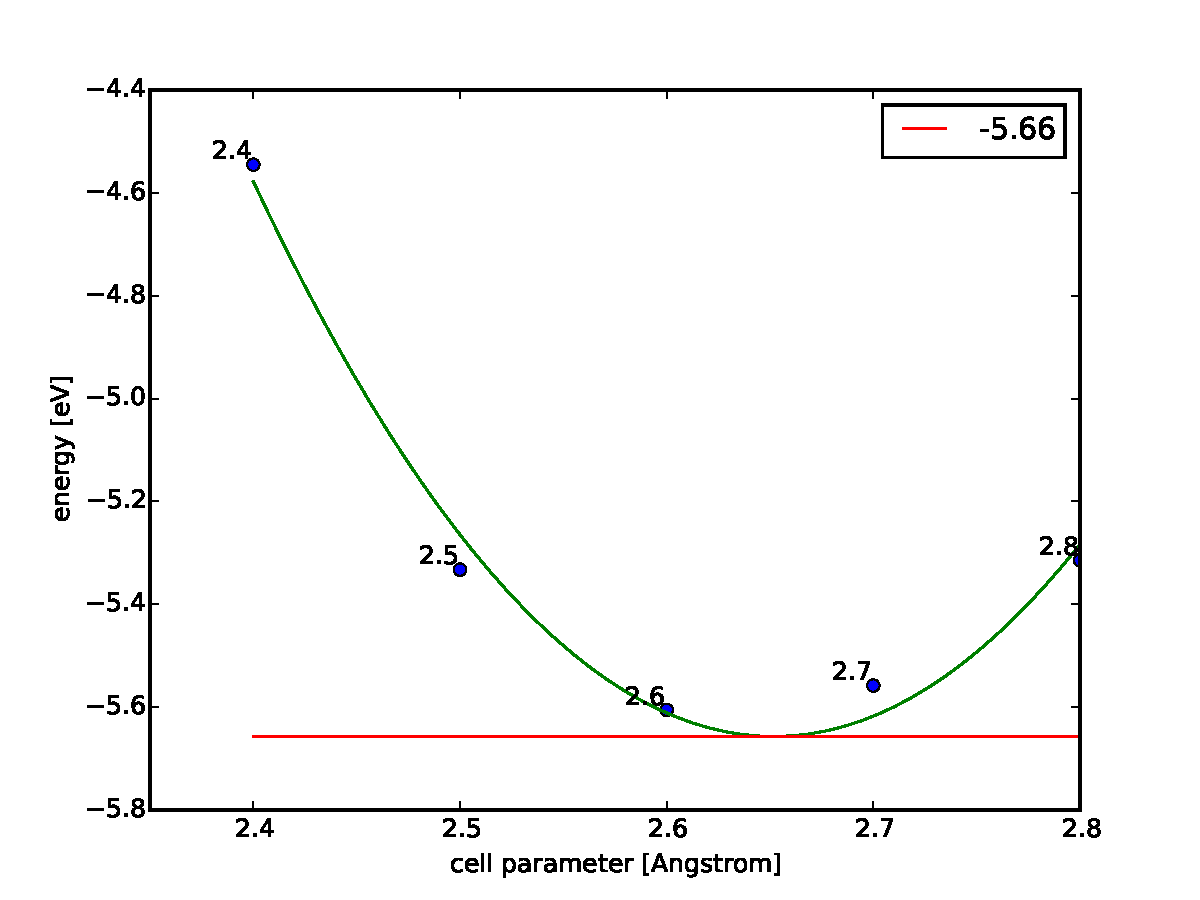
\includegraphics[width=0.7\linewidth]{sc}
	\caption{Total energy for different cell parameters for the simple cubic (\textbf{SC}) crystal system}
	\label{fig:sc}
	
	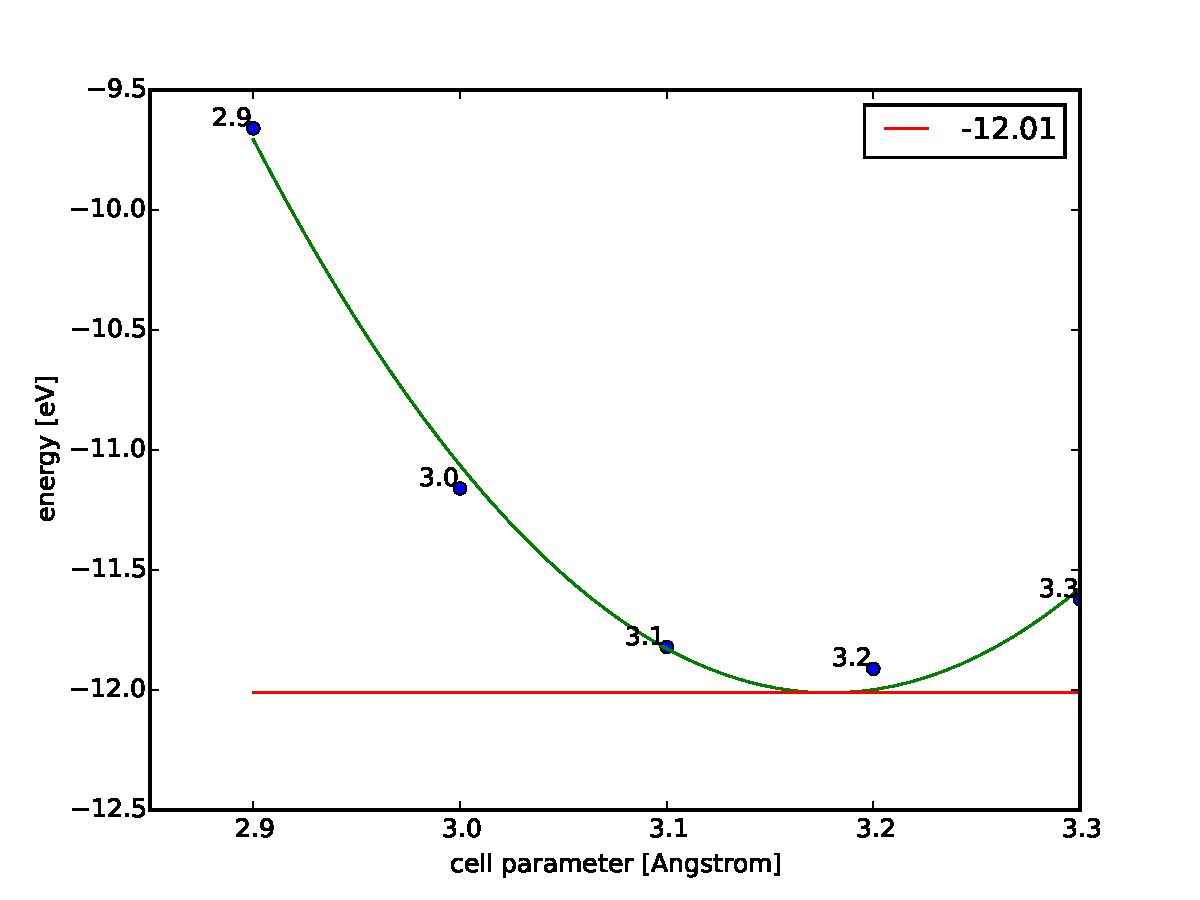
\includegraphics[width=0.7\linewidth]{bcc}
	\caption{Total energy for different cell parameters for the body centered (\textbf{BCC})crystal system}
	\label{fig:bcc}
\end{figure}
\begin{figure}[H]
	\centering
	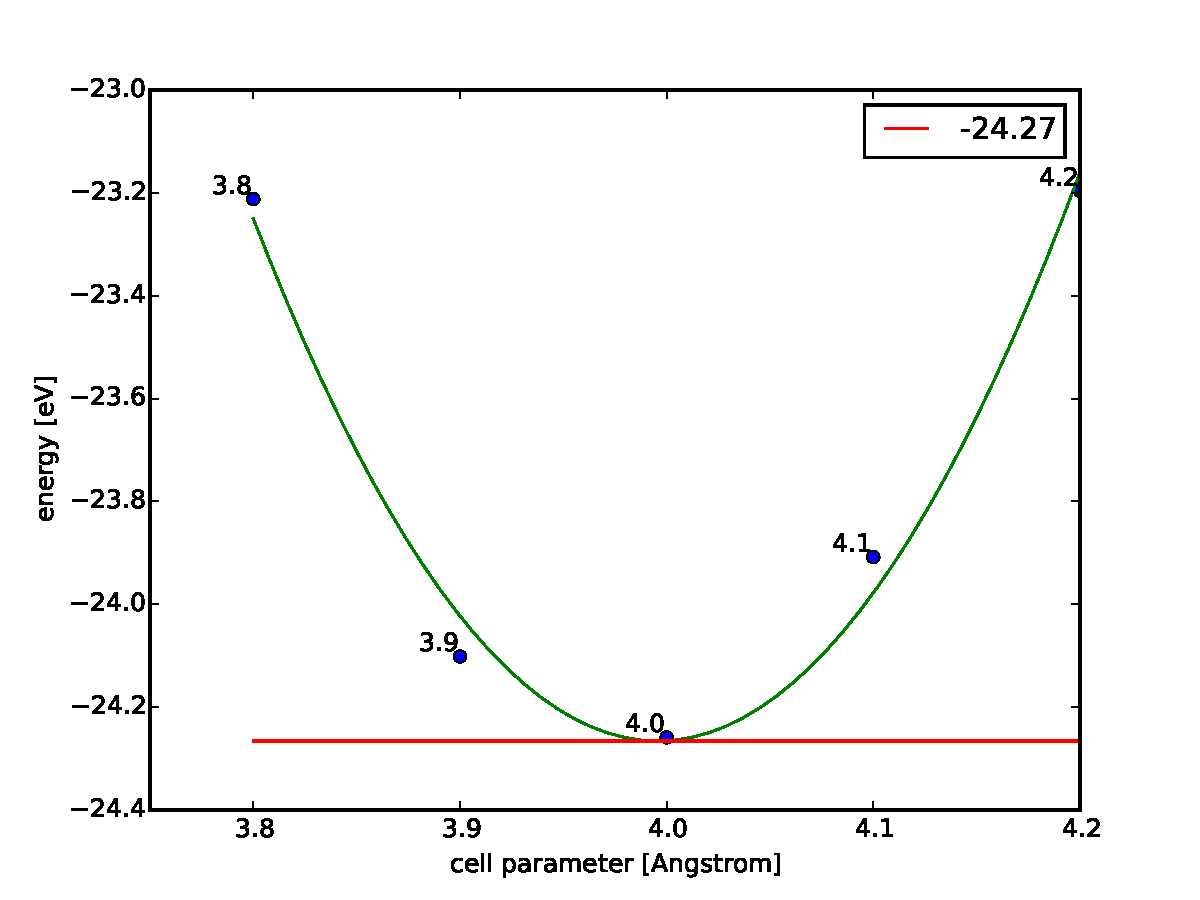
\includegraphics[width=0.7\linewidth]{fcc}
	\caption{Total energy for different cell parameters for the face centered cubic (\textbf{FCC})crystal system}
	\label{fig:fcc}
	
	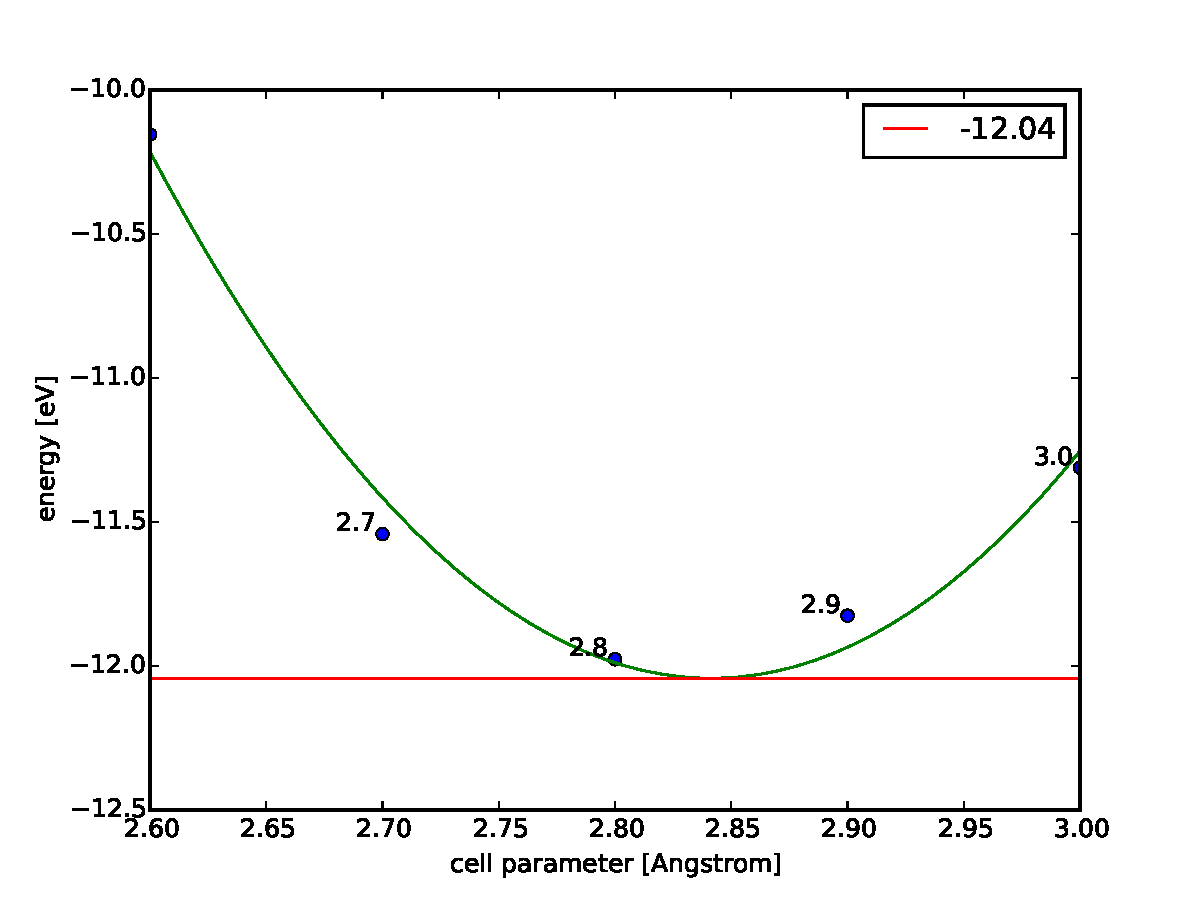
\includegraphics[width=0.7\linewidth]{hcp}
	\caption{Total energy for different cell parameters for the hexagonally close packed (\texttt{HCP}) crystal system}
	\label{fig:hcp}
\end{figure}
As should be the case we see that there is a minimum generated, the energy is minimized for some cell parameter. What this parameter is varies greatly, even when comparing the fcc and hcp, which has roughly the same energies, the cell parameters are very different. This is quite surprising
\section{Conclusion}
The results correlate very well with each other between the two different experiments. Almost exactly the same energies were found. By doing a parallell experiment like this, with different methods, the results validity is increased when they correlate. Platina is reported of having an fcc crystal structure. This agrees with the fact that we found a strong stability of fcc compared to sc and bcc. However, our prediction was that hcp was the most stable conformation for platinum. But it should be mentioned that they were quite close in energy, so only a small simplification in the modeling could have lead to the discrepancy. For instance, we do not take temperature effects into account here.

\appendix
\section{Python script}
\lstinputlisting[language = python]{fitcurve.py}

\end{document}


